\documentclass[output=paper]{langsci/langscibook}
\author{Moreno Mitrović\affiliation{ZAS Berlin and Bled Institute}}
\title{Extraordinary second-position effects}

% \chapterDOI{} %will be filled in at production

\abstract{Thanks to \textcite{Roberts2010}, the second-position (2P) effect is
    given a natural explanation using narrow-syntactic utilities alone, resting
    on his notion of defectivity. In this paper, I review and extend a
    narrow-syntactic approach to some other types of 2P effects that have, as
far as I know, not been studied in tandem; particularly extraordinary 2P
effects involving a combination of 2P placement and left branch extraction
(LBE).}

\maketitle

\begin{document}\glsresetall

\section{Introduction}

Thanks to \citet{Roberts2010}, the second-position (\textsc{2p}) effect is
given a natural explanation using narrow-syntactic utilities alone, resting on
his notion of defectivity. In this paper, I review and extend a
narrow-syntactic approach to some other types of \textsc{2p} effects that have,
as far as I know, not been studied in tandem; particularly extraordinary
\textsc{2p} effects involving a combination of \textsc{2p} placement and
\gls{LBE}.

There is no single treatment and theory of  all \textsc{2p} effects:
\textsc{2p} typology comprises at least three classes, based on the categorial
\emph{size} properties of the \textsc{1p} prima facie \enquote{hosting}
element. The first is the one where the host is a maximal category~-- these
constructions are exemplified by verb-se\-cond (\textsc{v2}) or
\gls{LBE}\is{left branch extraction} phenomena. The second type involves a host
of minimal category and are demonstrated by V-fronted constructions (e.g., long
head movement\is{head movement} in \ili{Breton}, V-topicalisation in Slavonic,
etc.). Both these types are discussed on a par and given a uniform treatment in
\citet{Roberts2010}.  The last type features non-constituent hosts comprising
of a head, say a preposition, and a maximal category, say an AP.  This last
type is incarnated by what \citet{Boskovic:2005} calls extraordinary
\gls{LBE}\is{left branch extraction} (XLBE). It is this last type that is most
resistant to narrow-syntactic explanation and, as far as I can gather from the
literature, no definitive and purely syntactic account has been proposed.

I aim to derive the last type of \textsc{2p} effect using
\posscitet{Chomsky2001} triadic characterisation \isi{movement} that
\citet[208]{Roberts2010} restated in parametric format (\ref{par}):

\begin{exe}
    \ex
	\begin{tabular}[t]{lccc|l}
             & Move & \isi{Agree} & Pied-pipe\\
		a.   & $+$  & $+$   & $+$         & A-movement \\
		b.   & $+$  & $+$   & $-$         & incorporation \\
		c.   & $+$  & $-$   & $+$         & Ā-movement \\
		d.   & $-$  & $+$   & $-$         & \isi{Agree} \\
		e.   & $-$  & $-$   & $-$         & $\emptyset$  \\
		f.   & $-$  & $+$   & $+$         & * \\
		g.   & $-$  & $-$   & $+$         & * \\
		h.   & $+$  & $-$   & $-$         & Ā-incorporation\\
	\end{tabular}
\label{par}
\end{exe}

If all three operations apply in tandem, A-movement obtains, while a
combination of Move and Pied-piping\is{pied-piping} along yield Ā-movement (with the absence of
an \isi{Agree} operation in Ā-processes being highly problematic). Head \isi{movement}, on
the other hand, can be seen as deriving from a combination of \isi{Agree} and Move.
While options (f) and (g) are impossible, by virtue of the axioms of Minimalist
syntax \citep{CollinsStabler:2016}, \citet{Roberts2010} takes the last
option  as corresponding to predicate clefting\is{clefts} or
Ā-in\-cor\-po\-ra\-tion.\footnote{For further empirical evidence of
Ā-in\-cor\-po\-ra\-tion, see \citet{Mitrovic:2017LIpa} and those he cites.} This
paper shows that this last  \isi{movement} operation  derives XLBE.

\citet[421]{Roberts2010} defines \glspl{IFF} on terminals in the clausal spine,
which are provided in \Cref{form-fs} along with corresponding \glspl{IFF} in
the nominal domain.
\glsreset{IFF}

\begin{table}
        \begin{tabular}{llll llll}
        \lsptoprule
        \multicolumn{4}{c}{in the verbal domain} & \multicolumn{4}{c}{in the nominal domain}\\\cmidrule(lr){1-4}\cmidrule(lr){5-8}
          C\tsp{min}  & $[i\textup{C}]$ & $[i\textup{T}]$  & $[i\textup{V}]$  &        P\tsp{min}  &   & $[i\textup{D}]$ &  $[i\textup{N}]$\\
          T\tsp{min}  &   & $[i\textup{T}]$ &  $[i\textup{V}]$             &        D\tsp{min}  &   & $[i\textup{D}]$ &  $[i\textup{N}]$\\
          \emph{v}\tsp{min}  &   &  & $[i\textup{V}]$                      &        $n^{\text{min}}$  &   &  & $[i\textup{N}]$\\
          V\tsp{min}  &   &  & $\emptyset$                               &        N\tsp{min}  &   &  & $\emptyset$                 \\
          \lspbottomrule
        \end{tabular}
        \caption{\Glspl{IFF}\label{form-fs}}
\end{table}

I assume that prepositions have no \gls{IFF} other than N and D. By adopting
the view that the presence of the (phasal) D head is subject to
cross-linguistic parametrisation, languages lacking the D-structure will
correspondingly have prepositions with only one \gls{IFF}, i.e. N.

The remainder of this section is devoted to explicating some background
assumptions and introducing the relevant discussion within which the analysis
is couched. After a brief survey of explananda for \textsc{2p} effects
(\Cref{subsec:2Peff}), the preliminary details of the N/D parameter of
\citet{Boskovic:2005,Boskovic2008}, which I am going to assume, are given in
\Cref{subsec:N-D}. Finally, in \Cref{subsec:def}, I outline the defectivity
system of \citet{Roberts2010} that underlies the account proposed here.
\Cref{subsec:road} provides the reader with directions I take in the following
sections.

\subsection{The \textsc{2p} effect and its explananda}\label{subsec:2Peff}

There are two general stances to explaining cliticisation\is{clitics}
phenomena. By the end of this subsection, I hope to demonstrate that one of
these approaches should be preferred on both theoretical and empirical grounds.

One of the foundational questions concerning \textsc{2p}
cliticisation\is{clitics} phenomena is: Where does cliticisation\is{clitics}
take place? At least two answers have been around for decades: either
cliticisation\is{clitics} configurations are established and derived in narrow
syntax (NS) or, otherwise, they are epiphenomenal and reflective of
post-syntactic (or more precisely phonological or prosodic) displacement and
rearrangement. Let me briefly lay out a two-tiered motivation for preferring
the former over the latter.

A phonological/prosodic (i.e., ``anti-syntactic'') motivation for
second-position (\textsc{2p}) cliticisation\is{clitics} is most notably and
influentially characterised by the theory of \gls{PI} as advocated by
\citet{Halpern:1992,halpern:1995dq}. As \citet[422]{roberts:2012uq} notes,
there are three ingredients to this theory as given in (\ref{PI-ingr}).

\begin{exe}
\ex
\begin{xlisti}
\ex \textsc{2p} \isi{clitics} are prosodically subcategorised to appear right-ad\-ja\-cent to a prosodic word; \label{PI-i}
\ex \isi{clitics} adjoin to IP; \label{PI-ii}
\ex where no element with a phonological matrix appears to the left of the
IP-adjoined clitic, then \gls{PI} must apply, in line with (\ref{PI-sketch}).
\label{PI-iii}
\end{xlisti}
\label{PI-ingr}
\ex \textsc{clitic} $>$ $X$ $>$ $Y$ $\longrightarrow$  $X$ $>$ \textsc{clitic} $>$ $Y$

\label{PI-sketch}

\end{exe}

Given a relevant prosodic domain, the clitic and the rightmost element thus
prosodically flip and the second-position effect obtains (\ref{PI-sketch}), in
line with the principles in (\ref{PI-ingr}). Note, however, that
(\ref{PI-sketch}) is a sketch and there are certainly works within this
approach where \textsc{2p} \isi{clitics} are located in positions other than
IP. (For a detailed overview and a summary of all relevant arguments, I refer
the reader to \citealt[75ff]{Boskovic:2001b} and citations therein.)

Let me now review some arguments that undermine the nature of such
principles.\footnote{In doing so, I also adopt the rationale of
\citet[422]{roberts:2012uq}.} Firstly, with respect to (\ref{PI-i}), the
\textsc{2p} order may be derived using more general syntactic principles, as  I
will demonstrate. Additionally, categorising an element as, and assigning it a
descriptively arbitrary label of, a clitic is extraneous insofar as the
\enquote{clitic effect} may arise from the configuration of the clitic with
respect to other elements, especially its \enquote{host}. Secondly, and in
connection to (\ref{PI-ii}), it is not only stipulative but also
counter-theoretical to assume that \isi{clitics} adjoin to IP. On the one hand, the
current minimalist  model of phasal syntax demonstrably takes the C$^0$, and
not the T$^0$, head to be a phase\is{phases} head and, as such, the locus of
clitic-clustering should be on phase\is{phases} heads, i.e. C$^0$ and \emph{v}\tsp{0} (I
demonstrate the conceptual and empirical connection between cliticisation\is{clitics}
target sites and the phasal nature of such sites below but see
\citet{Roberts2010,roberts:2012uq} for a detailed account and motivation).  An
additionally problematic conception of (\ref{PI-ii}) concerns the nature of
\enquote{adjunction}\is{adjunction} which cannot be maintained in line with the standard
assumptions of syntax. This proviso of \gls{PI} predicts all \isi{clitics} to either
be base generated at IP-level or internally moved to an IP-level adjunct
position.  Consider empirical instances of DP-level conjunction \isi{clitics} in
\ili{Indo-European} (e.g.\ \ili{Latin} \emph{-que}, or \ili{Hittite} \emph{-a}) or, say, object
\isi{clitics} in \ili{Romance} or South Slavonic in relation to this proviso. The amount of
stipulation that would ensue if I assume there exists \isi{movement} of a DP
conjunction in the former example or object DP in the latter in order to render
the syntactic conditions for \gls{PI} to apply, in line with (\ref{PI-ii}),
would be too great for a theory of syntax to remain consistent.

On a more general level, the existence of a stru\-cture-tampering operation,
such as \gls{PI} as formulated above, breaches the basic tenets of the
minimalist linguistic theory or, at least, cannot be defined in  accordance
with the general minimalist assumptions. Since the \isi{Merge} operation derives
syntactic structures and the nature of \isi{movement} operations, it has to be
confined to the core syntactic module of grammar. I thus cannot maintain this
theoretical principle and expect to find displacement operations, derived by
Merge, outside the modular confines of syntax.

A less general and more damaging evidence against \gls{PI} is empirical. I
briefly provide an argument coming from Ser-Bo-Croatian\il{Serbo-Croatian}
\glspl{LBE}. \citet{Boskovic:2009b}, among others, convincingly shows that
\gls{PI} cannot account for the following morphosyntactically conditioned
violations of the \gls{LBC}. While non-extracted DPs containing both forenames
and last names allow the forename to be unmarked for case, a left-branch
extracted\is{left branch extraction} forename must obligatorily be case-marked;
in the case of (\ref{leo1}), as an accusative.

\begin{exe}
\ex Ser-Bo-Croatian\il{Serbo-Croatian}
\begin{xlista}
\ex
\begin{xlisti}
\ex[]{\gll Lav-a Tolstoj-a sam čitao	 \\
Leo-\Acc{} Tolstoy-\Acc{} \Aux.\Fsg{} read.\textsc{ppl.sg.m} \\
\trans `I'm reading Leo Tolstoy.'}

\ex[]{\gll Lav Tolstoj-a sam čitao	 \\
Leo-\Nom/∅ Tolstoy-\Acc{} \Aux.\Fsg{} read.\textsc{ppl.sg.m} \\
\trans `I'm reading Leo Tolstoy.'}

\end{xlisti}

\ex
\begin{xlisti}
\ex[]{\gll Lav-a sam Tolstoj-a čitao	 \\
Leo-\Acc{} \Aux.\Fsg{} Tolstoy-\Acc{} read.\textsc{ppl.sg.m} \\
\trans `I was reading Leo Tolstoy.'}

\ex[*]{\gll Lav sam Tolstoj-a čitao	 \\
Leo-\Nom/∅ \Aux.\Fsg{} Tolstoy-\Acc{} read.\textsc{ppl.sg.m} \\
\trans `I was reading Leo Tolstoy.'}
\end{xlisti}

\end{xlista}
	\label{leo1}
\end{exe}

If some post-syntactic algorithm did in fact derive \gls{PI}, it is nearly
impossible to account for the empirical facts stated above without having the
phonological-prosodic module of grammar be sensitive to narrow morphosyntactic
properties or features such as case marking.

Also consider the fact that it is not \isi{clitics} alone that may interrupt a
complex DP, such as the \enquote{Leo Tolstoy}-type compounds names above. As
\citet{Boskovic:2009b} observes, a non-clitic item, such as a full finite
lexical verb \emph{čitam} `read.\Fsg.\Prs{}', may also break up the name
(\ref{leo2}). In line with \citet{roberts:2012uq}, I assume that the first-name
D\tsp{max} Ā-moves to the position of Spec(Force\tsp{max}) with the full verb
remaining in T\tsp{min}. Note further the obligatory case-marking on the
extracted forename DP.

\begin{exe}
    \ex Ser-Bo-Croatian\il{Serbo-Croatian}\\
    \gll Lava čitam Tolstoja \\
    Leo.\Acc{} read.\Fsg.\Prs{} Tolstoy.\Acc{} \\
    \trans `I'm reading Leo Tolstoy.'
\label{leo2}
\end{exe}

Furthermore, the following is also well-formed, which lends empirical support
to \posscitet{Roberts2010} motivation that Ā-movement of minimal categories
should exist. The continued range of cases of clitic interruptions of the
first-last-name DP should amplify empirically this argument.

\begin{exe}
\judgewidth{(?)}
    \ex Ser-Bo-Croatian\il{Serbo-Croatian}
\begin{xlista}
\ex[(?)]{ \gll Lava sam čitao Tolstoja \\
Leo.\Acc{} \Aux.\Fsg{} read.\textsc{ppt.sg.m} Tolstoy.\Acc{}\\
\trans `I (have) read Leo Tolstoy.'
}
\ex[(?)]{ \gll Lava  čitao sam Tolstoja \\
Leo.\Acc{} read.\textsc{ppt.sg.m} \Aux.\Fsg{}  Tolstoy.\Acc{}\\
\trans `I (have) read Leo Tolstoy.'}
\end{xlista}
\label{6}
\ex Ser-Bo-Croatian\il{Serbo-Croatian}
\begin{xlista}
\ex[]{ \gll Lava mi je Tolstoja dao da čitam\\
Leo me.\Dat{} is Tolstoy gave that read.\Fsg.\Prs{}\\
\trans `He gave me Leo Tolstoy to read.'}
\ex[]{\gll Lava sam joj Tolstoja dao da čita\\
Leo am her.\Dat{}  Tolstoy gave that read.\Ssg.\Prs{}\\
\trans `I gave her Leo Tolstoy to read.'}
\ex[]{ \gll Lav si je Tolstoj (sam) doručak pravio \\
Leo self.\Dat{} is Tolstoy (himself) breakfast made\\
\trans `Leo Tolstoy (himself) made himself breakfast.'}
\end{xlista}

\end{exe}

Note that some speakers concede that (\ref{6}b) is degraded without a pause
following \emph{Lava}. The requirement for the pause is captured prosodically
by a generalisation that Ser-Bo-Croatian\il{Serbo-Croatian} \textsc{2p}
\isi{clitics} must be second within their intonational phrase \citep[65, n.\
120]{Boskovic:2001b}. The account I provide is consistent with this
generalisation as I advocate a view that NS movement coincides with
intonational phrasing.

If the theory of \gls{PI} cannot account for the contemporary \gls{LBE}\is{left
branch extraction} phenomena found in Ser-Bo-Croatian\il{Serbo-Croatian}, I
inductively find it untenable to entertain this theory as general explanandum
applicable to a cross-lin\-gui\-stic patterns of cliticisation\is{clitics} which also
display \gls{LBC}\is{left branch condition} violations. On grounds of both
theoretical and empirical motivation, I thus pursue a NS aetiology of
cliticisation, also for reasons of more general parsimony, as noted by
\citet[73--74]{Roberts2010}; namely I choose, and logically prefer, not to
accord extra-syntactic factors too prominent a role  in order to maintain the
approach in full generality. It is thus, ceteris paribus, more
theoretically consistent to adhere to  the central syntactic account and derive
a maximally possible account of the distribution of facts from that.

More specifically, since a NS account of cliticisation\is{clitics} does not suffer from the
two drawbacks stated above, I am lead to maintain this assumption in the
analysis.

\subsection{The N/D parameter}\label{subsec:N-D}

With background notions in place, I discuss in the remainder of the paper how
the relation between the N/D parameter and the system of defectivity can be
married in an analysis of XLBE.

Assuming that D\tsp{max} constitutes a phase\is{phases}, \citet{Boskovic:2005}
provides an account of why some languages allow and others disallow
\gls{LBE}\is{left branch extraction}.\footnote{See \citet{Boskovic:2013} for a
more recent and phase-based discussion of \gls{LBE}\is{left branch
extraction}.} Given that D\tsp{min} is a phase\is{phases} head, it prohibits
movement of its complement with only its edge being accessible as per the PIC.
His first assumption is that languages like Ser-Bo-Croatian\il{Serbo-Croatian} lack the D-layer in
their nominal spine and, due to this, lack a nominal phase\is{phases}, making their
interior accessible. His second assumption is that adjunction structures\is{adjunction} come
in two parametric options: either the adjective takes an NP complement
(AP-over-NP) or the AP is adjoined to NP (NP-over-AP).\is{adjunction}

Consider a scenario of AP-extraction in \ili{English} which is barred due to the
presence of the phasal D. In order for AP to extract, it must pass through D's
edge, i.e. Spec(D\tsp{max}). This, however, is an anti-local move and thus
prohibited by the independently motivated principles of grammar. Thus, the
combination of the PIC and anti-Locality bans \gls{LBE}\is{left branch
extraction} in D-containing language like \ili{English}.

By contrast, \citet{Boskovic:2005,Boskovic2008} contends that
Ser-Bo-Croatian is a D-less language in which nominals are not phasal, hence
the PIC is inapplicable. Consequently, there is no need for anti-local moves of
the AP since the AP may immediately and directly extract to the final position.
This is the line of reasoning I will adopt on both empirical and theoretical
grounds.

\subsection{Defectivity}\label{subsec:def}

The second and more foundational is the assumption surrounding triggers of
head-movement.\is{head movement} \posscitet{Roberts2010} system predicts
incorporation to take place where an \isi{Agree} relation holds between a probe
and a goal such that the formal features of the goal form a proper subset of
the features specified on the probe. This constitutes the goal as defective and
such goals incorporate.  The concept of defectivity thus regulates
\isi{movement} of the minimal category.

\begin{exe}
\ex \textsc{defectivity} \citep{Roberts2010}\\
A goal G is defective iff G's formal features are a proper subset of those of G's probe P.
\end{exe}

Thus, in more formal terms, a set of formal features (F) on a minimal category
that enters an \isi{Agree} relation as a Probe (P) will incorporate the Goal
(G) iff (\ref{def-form}) is met.

\begin{exe}
    \ex F\tss{G} $\subset$ F\tss{P}
\label{def-form}
\end{exe}

For instance, \ili{Romance} pronominal objects \isi{clitics} are taken to
correspond to φ\tsp{min/max}, lacking a D feature. The \emph{v}\tsp{min},
bearing an \gls{IFF} $[i\textsc{V}]$ (\tabref{form-fs}),  probes
for valuing its [\emph{u}φ]. Upon valuation, $F_G \subset F_P$ holds and the
object φ\tsp{min/max} incorporates into \emph{v}\tsp{min}. As
\citet[391]{roberts:2012uq} further notes, ``[t]his means that the Match
relation holding in virtue of Agree causes the host to become a featural copy
of the probing features of the host.'' The chain reducing algorithm that
applies post-syntactically, and which ensures economical assignment of
phonological indices, will treat the host-probe and the defective clitic-goal
as a single feature bundle. Thus, for a chain \[\tuple{[G+P],\emph{t}\tss{G}}\]
the algorithm will pronounce the head of the chain only, giving the effect of
\isi{movement}.

By contrast to \ili{Romance}, Slavonic \isi{clitics} are not \emph{v}-oriented
but cluster in the C-domain. \citet{Roberts2010} derives the C-orientation by
positing that Slavonic \isi{clitics} are not φ\tsp{min/max} elements (since
they would be \emph{v} in\-cor\-po\-ra\-ting otherwise) but D\tsp{min/max}.
Since \emph{v}\tsp{min} has no uninterpretable D-feature, these \isi{clitics}
can thus escape incorporating into \emph{v}.\footnote{On the escape system, see
\citet[391--392]{roberts:2012uq} and references there.} By virtue of C's
bearing an uninterpretable D-feature, pronominal D\tsp{min/max} elements (as
well as D-bearing auxiliaries sitting in T\tsp{min}) cliticise onto C.

In conclusion to this section, consider the apparent contradiction that arises
in our assuming the systems of \citet{Roberts2010} and \citet{Boskovic:2005}.
For \citet{Roberts2010}, it is critical that pronominal \isi{clitics} in
Ser-Bo-Croatian\il{Serbo-Croatian} be D\tsp{min/max}. For \citet{Boskovic:2005},
on the other hand, Ser-Bo-Croatian\il{Serbo-Croatian} has no D category. I
propose to reconcile the two approaches, in their assumptions and conclusions,
by treating Ser-Bo-Croatian\il{Serbo-Croatian} pronominal \isi{clitics} not as
D elements but as making up N\tsp{min/max}. To maintain the defectivity
approach of \citet{Roberts2010}, I take the C\tsp{min}, conversely, as being
specified with a $[u\textsc{N}]$.

This view of subsuming the N/D parameter alongside a defectivity-based system
of explananda which require me to adjust some of the basic assumptions and
tenets of \citet{Roberts2010}. As preliminarily discussed  in the following
subsection, this is a fully compatible view which expands the explanatory
adequacy of the defectivity approach and helps resolve XLBE.

\subsection{Desiderata and roadmap}
\label{subsec:road}

In the previous two subsections, two seemingly orthogonal ideas were laid out:
a parametric and a presumably universal one. The former concerns the choice
between encoding arguments as N- or D-elements. The latter concerns defectivity
conditions defined on an \isi{Agree} operation between objects bearing formal
features which, when met, legislate incorporation of the goal into the probe.

The two views, while appealing to different derivational devices and
conditions, are seemingly incompatible as one assumes that \isi{clitics} are
D-elements \citep{Roberts2010} while another opposes this view
\citep{Boskovic:2009b}.

The primary desideratum is to derive a narrow-syntactic analysis of the
word-first \textsc{2p} effect by suggesting that the effect derives from
constituent-only consideration, as opposed to (linearity-based) word-level
\enquote{counting} which phonological explananda suppose.

Secondarily, I will restate the N/D parameter in terms of the defectivity
technology that applies to a pair in an \isi{Agree} relation, rather than general
structural edge- or barrier-based restrictions on extraction domains.  This
will show that the N/D split theory is compatible with the defectivity approach
to head \isi{movement}.\is{head movement}

The scope of this paper is largely restricted to achieving the first
desideratum, with the second one requiring apparent abandonment of the
assumptions made in the previous subsection, especially in connection to
defectivity. \Cref{sec:phase}, however, outlines a resolution for the
question of how the defectivity approach may be integrated with the N/D
parameter.

In \Cref{sec:shimada} I outline a technical assumption which will allow me to
combine the N/D and cliticisation\is{clitics} parameters. In \Cref{sec:deriv}, a second
position typology is presented with the empirical core of XLBE, which is
analysed in \Cref{sec:xlbe}. \Cref{sec:phase} provides a programmatic post hoc
outlook on rectifying the counterintuitive assumption on the internal structure
of \isi{clitics} in South Slavonic. I essentially appeal to a parametric recasting of
the nature of the relevant \gls{IFF} in pronominal \isi{clitics} which would yield
the two core taxonomies, C- and \emph{v}-oriented \isi{clitics}, while
retaining the view that South Slavonic pronominal \isi{clitics} are not
D-elements, in line with the tenets of \citeauthor{Boskovic:2001b}
(\citeyear{Boskovic:2001b,Boskovic:2004c,Boskovic:2005,Boskovic:2009b}).  The
following section first provides another crucial piece of technology I rely on
in order to derive a narrow-syntactic analysis of XLBE.

\section{The unrolling spine: Shimada
\citeyearpar{Shimada:2007}}\label{sec:shimada}

While my account rests on the notion of defectivity as underlying
nar\-row-syn\-tac\-tic incorporation as per \citet{Roberts2010}, I add another
theoretical ingredient.

I follow \citet{Shimada:2007} in assuming that the clausal spine in fact
results from a successive unrolling or excorporation of a head verbal complex
that contains the entire clausal extended projection
\parencite[cf.][]{Saito:2012}. I assume that the label every branching
non-root  node in the head-complex lacks the label (λ). I define on the clausal
terminals their \glspl{IFF} along with the [\emph{u}φ] and $[u\textup{D}]$ at
phasal levels of \emph{v}\tsp{min} and C\tsp{min}, respectively (in line with
\citealt{Roberts2010}).

\begin{exe}
	\ex

	\hfill
    \begin{tikzpicture}[baseline=(root.base)]
        \Tree [.\node(root){V\tsp{max}}; \edge[dashed]; D\tsp{max} \edge[dashed]; [.{V\tsp{min}} {V\tsp{min}}  [.{λ} {\emph{v}\tsp{min}\\$[i\textup{V},u\phi]$}  [.{λ} {T\tsp{min}\\$[i\textup{V}, i\textup{T}]$}  {C\tsp{min}\\$[i\textup{V}, i\textup{T},i\textup{C},u\textup{D}]$}  ] ] ]]
	\end{tikzpicture}
	\hfill
\label{shimada1}
\end{exe}

Note that prior to excorporation of \textsc{Compl}(V\tsp{min}) in
(\ref{shimada1}), there is only one pair of terminals satisfying the
defectivity condition on incorporation: T\tsp{min} and C\tsp{min}. However, the
\gls{LCA}\is{Linear Correspondence Axiom} prohibits such \isi{movement}, making
incorporation inapplicable at this stage.\is{LCA|see{Linear Correspondence
Axiom}}

Once the V has combined with an argument, say D\tsp{max} (which has
undergone spine-unrolling), its complement, headed by \emph{v}\tsp{max},
excorporates to the root for two reasons: semantically, there is a
type-mismatch (hence the λ) and, perhaps more importantly for our
syntactic purposes, \textsc{Com\-ple\-ment}(V\tsp{min}) is lacking
a label. Once it excorporates, the c-selecting head, \emph{v}\tsp{min} projects
the label (\ref{3}).

\begin{exe}
	\ex
	\hfill
    \begin{tikzpicture}[baseline=(root.base)]
        \Tree [.\node(root){\emph{v}\tsp{min/max}}; [.\emph{v}$^{\text{min}}_1$  {\emph{v}\tsp{min}\\$[i\textup{V},u\phi]$} [.λ {T\tsp{min}\\$[i\textup{V}, i\textup{T}]$} {C\tsp{min}\\$[i\textup{V}, i\textup{T},i\textup{C},u\textup{D}]$} ]] [.V\tsp{max} \edge[dashed]; λ\tss{1} [.V\tsp{max}  D\tsp{max} [.V\tsp{min} \edge[dashed]; V\tsp{min} \edge[dashed]; $t_1$  ] ] ]]
	\end{tikzpicture}
		\hfill
\label{3}
\end{exe}

Given the strong cycle, V\tsp{min}-incorporation takes place as well as
External \isi{Merge} of the argument, checking [\emph{u}φ] on
\emph{v}\tsp{min}. In the next derivational step, the remaining λ-complex
containing T\tsp{min} and C\tsp{min} excorporates for the same reasons I gave
earlier. The result, after subject \isi{raising} (\Sbj) and final excorporation
of C\tsp{min} from the T-complex, viz.\ the structure in \figref{fig:18.1}.
%\tuple{C$^{min}_{3}$,\lambda$_3$,t$_3$} chain, yields the

\begin{figure}
\caption{A clause-unfolding analysis utilising successive excorporation
\parencite{Shimada:2007}\label{fig:18.1}}
    \resizebox{\textwidth}{!}{\begin{tikzpicture}[baseline=(root.base), align=center]
        \Tree
            [.\node(root){C\tsp{max}};
                {C$^{\text{min}}_{3}$\\
                {}[\emph{i}V, \emph{i}T, \emph{i}C,\emph{u}D]}
                [.T\tsp{max}
                    \edge[dashed]; λ\tss{3}
                    [.T\tsp{min/max}
                        \edge[dashed]; D$^{\text{max}}_{\Sbj{}}$
                        [.T\tsp{max}
                            [.T$^{\text{min}_{2}}$
                                {T\tsp{min}\\
                                {}[\emph{i}V, \emph{i}T]}
                                \edge [dashed]; \emph{t}\tss{3}
                            ]
                            [.\emph{v}\tsp{max}
                                λ\tss{2}
                                [.\emph{v}\tsp{max}
                                    \emph{t}\tss{\Sbj}
                                    [.\emph{v}\tsp{min/max}
                                        [.\emph{v}$^{\text{min}}_{1}$
                                            {\emph{v}\tsp{min}\\{}[\emph{i}V, \emph{u}φ]}
                                            \emph{t}\tss{2}
                                        ]
                                        [.V\tsp{max}
                                            \edge [dashed]; λ\tss{1}
                                            [.V\tsp{max}
                                                D\tsp{max}
                                                [.V\tsp{min}
                                                    \edge [dashed]; V\tsp{min}
                                                    \edge [dashed]; t\tss{1}
                                                ]
                                            ]
                                        ]
                                    ]
                                ]
                            ]
                        ]
                    ]
                ]
            ]

    \end{tikzpicture}}
\end{figure}

The resulting derivation is identical to the standardly assumed one, hence
standard operations, including A- and Ā-processes, apply. I will tacitly assume
in the remainder of the paper that the spine unrolls along the lines just
sketched and, therefore, use a traditional and simplistic drawing of the trees.
In \Cref{sec:xlbe}, the details of the assumptions concerning the
excorporational onset of derivations will become clear.

\section{Deriving the phrase-/head-first \textsc{2p} effect}
\label{sec:deriv}

In this section, I provide a derivational account of constituent-first
\textsc{2p} effects. In \Cref{subsec:X1}, I sketch an account of Wackernagel
effects found across old IE conjunction structures which feature a minimal
category as the host of enclisis. I turn to hosts of maximal categories in
\Cref{subsec:XP1}, and, lastly, to a phenomenon which seems to alternate
between phrase/head-first in Slavonic in \Cref{subsec:XP-X1}.

Note however, that the empirical locus of paper lies in XLBE
(\Cref{subsec:XP-X1}). While other phenomena, including \textsc{v2} and
V-topicalisation\is{topicalization} may well be analysed using the same principles of the
derivation I adopt and propose, these fall outside of the scope of the present
paper.\footnote{For an analysis of \textsc{v2}, compatible with the
spine-unrolling tenets, see \citet[Ch. 2]{Shimada:2007}. For an analysis of
V-topicalisation,\is{topicalization} see \citet{CavarWilder:1992}, \citet{Mitrovic:2017pa}, among
others.}

\subsection{X-first}\label{subsec:X1}

Word-first constructions are a wide-spread phenomenon in old IE
\isi{coordination} structures and were first described by
\citet{wackernagel:1892jl}. I cite below three examples from Old Irish
(\ref{oir}), Gothic (\ref{got}) and Old Avestan (\ref{avs}). \footnote{For a
detailed view, see \citeauthor{Mitrovic:2014phd}
\citeyearpar{Mitrovic:2014phd,Mitrovic:2019}, and references therein.}

\begin{exe}
    \ex \ili{Old Irish}; \emph{Laws}, 4.179 \parencite{thurneysen:2003dq}\\
    \gll \ldots{} ba  \textbf{{\.{c}}}  ri Temrach \\
    {} \Cop{} and king Tara.\Gen{} \\
	\trans `And he was king of Tara.'\label{oir}
    \ex \ili{Gothic}; \emph{Codex Argenteus}, Jn. 18:33\\
    \gll wopida Iesu qa{þ} \textbf{{uh}} imma. \\
	called.\Prt.\Tsg{} J.\Acc{} said.\Prt.\Tsg{} and him.\M.\Dat.\Sg{} \\
    \trans `(Then Pilate entered into the judgment hall again, and) called Jesus, and said unto him.'\label{got}
    \ex \ili{Old Avestan}; \emph{Yasna Haptanghāiti}, 29.10\\
    \gll yūžəəm aēibiiō ahur{ā}  aog{ō} d{ā}t{ā} a{\d{š}}{ā} x{\d{š}}aϑrəm \textbf{{c{ā}}} \\
    you.\textsc{2.sg.nom} them.\textsc{pl.dat} lord.\textsc{m.sg.voc} strength.\textsc{n.sg.acc} give.\textsc{2.pl.aor.imp} truth.\textsc{n.sg.inst} power.\textsc{n.sg.acc} and \\
    \trans	`O Lord, may you give strength to them through truth and that power [\ldots]' \\
\label{avs}
\end{exe}

The common pattern that emerges in these coordinate
constructions\is{coordination} is that
there is exactly one word preceding the conjunction maker. Assuming a
J(unc\-tion) structure, I take this one-word precedence to derive from
head-movement\is{head movement} from within the internal (second) conjunct:

\begin{exe}
\ex
    \begin{tikzpicture}[baseline=(root.base)]

        \Tree
            [.\node(root){J\tsp{max}};
                α\tsp{max}
                [.J\tsp{min/max}
                    [.J\tsp{min}
                        {X\tsp{min}$\in$ β\tsp{max}}
                        J\tsp{min}
                    ]
                    β\tsp{max}
                ]
            ]

    \end{tikzpicture}
\end{exe}

Coordination structures of this type are semantically unmarked across all old
IE languages. Since incorporation into the coordinator is consistently blind to
the category of the incorporee, Ā-incorporation would appear as the best
candidate for an explanandum. This would require positing some Ā-feature such
as [\gls{EF}]  on J\tsp{min}, making it phasal in nature.
Assuming that it lacks a categorial label (see \citealt{Chomsky2013},
inter alia), J\tsp{min} has some \gls{IFF} and an
uninterpretable categorial feature  which is checked via c-selection. Note that
its bearing an uninterpretable feature makes  J\tsp{min}
potentially phasal in nature.\footnote{\citet{Mitrovic:2014phd} provides
semantic arguments for information-related properties of \textsc{2p} in IE,
lending support to the Ā-incorporation analysis.}

An alternative view to Ā-incorporation would be to adopt an Agree-based account
of incorporation. Assume J has no [\gls{EF}] specified, but does have a
category feature without a value, as per standard assumptions. Once valued,
every accessible minimal category in \textsc{Compl}(J\tsp{max}) is a
\isi{defective goal} and the closest one undergoes incorporation. (For a
synchronic and diachronic account of the syntax of \isi{coordination} in IE,
see \citealt{Mitrovic:2014phd,Mitrovic:2018oup,Mitrovic:2019}.)

Similar \textsc{2p} effect with a minimal category can be observed in Slavonic.
Unlike the Wackernagel data above, it is the pronominal \isi{clitics} that undergo
movement by virtue of their being defective goals.\is{defective goal} In Slavonic, pronominal
clitics are treated as D\tsp{min/max} which are probed by a
$[u\textsc{D}]$-car\-ry\-ing C (more precisely, Fin\tsp{min}). Once
incorporated, the C's [\gls{EF}], specified presumably on
Force\tsp{min}, is checked via Ā-movement to its edge (see
\citealt[386--399]{roberts:2012uq} and citations there for details).

\subsection{XP-first}\label{subsec:XP1}

The phrase-first \textsc{2p} effect is elegantly parallel to the head-first
\textsc{2p} effect. One difference is that in XP-first constructions, the
phasal [\gls{EF}] is checked by phrasal \isi{movement}.

The \ili{Germanic} \textsc{v2}-type falls into this category and differs minimally
from the Slavonic type in that, as \textcite[401]{roberts:2012uq} writes, while
Slavonic \textsc{2p} ``require[s] fronting of just one
element -- \emph{either} a head \emph{or} an XP -- the latter require
fronting of \emph{both} a \emph{head} and an XP.''

\subsection{XP/X-first}\label{subsec:XP-X1}

What follows is the core of this section: there are configurations which
seemingly alternate between X-first and XP-first. The constructions in question
concern Ser-Bo-Croatian\il{Serbo-Croatian} subject conjunctions (SCS).

The empirical focus of this section lies on the following pair of data:

\begin{exe}
	\ex Ser-Bo-Croatian\il{Serbo-Croatian}\\
    \gll $\big[$ Ja i Mujo $\big]$ smo otišli na pivo.\\
    {} I and M {} will.\Pl{} go.\Ptcp{} on beer \\
	\trans `Mujo and I are going for a beer.'
	\label{conj-sc1}
	\ex Ser-Bo-Croatian\il{Serbo-Croatian}\\
	\gll $\big[$ Ja smo i Mujo $\big]$  otišli na pivo.\\
    {} I will.\Pl{} and M {} go.\Ptcp{} on beer \\
	\trans `Mujo and I are going for a beer.'
	\label{conj-sc2}
\end{exe}

While (\ref{conj-sc1}) shows a plain vanilla subject conjunction structure, the
availability of (\ref{conj-sc2}) does not readily follow, prima facie,
from \posscitet{Roberts2010} tenets.  With regards to the conjunction
subject, the plural auxiliary\is{auxiliaries} verb \emph{ćemo}, once raised from
Aux\tsp{min} to T\tsp{min}, is in \textsc{2p} with
respect to the \emph{maximal} category linearly to its left. What
(\ref{conj-sc2}) shows, however, is that the Aux may be placed in a \textsc{2p}
with respect to the \emph{minimal} category -- I refer to this construction
as \textsc{second-word} (\textsc{2w}) effect. This very oscillation between word- and
constituent-second configurations raises the core question on how a
narrow-syntactic explanandum for seemingly string-related, and linearity-based,
behaviour may obtain.\footnote{For independent arguments against the view that
second-position effects derive from phonological processes, see \citet[11--36,
75--93]{Boskovic:2001b}, \citet[Ch. 3]{Roberts2010}, and further references
therein.}

On independent empirical grounds, then, we are led once more to reconsider the
\textsc{2p} effect with regards to the structural size of the
first-po\-si\-tion host.

While nominal \isi{clitics} in Ser-Bo-Croatian\il{Serbo-Croatian} are
D\tsp{min} elements that obligatorily incorporate into (some)
C\tsp{min} by virtue of defectivity, there is no defective relation
constituted by an \isi{Agree} chain between a clausal head and the verb, or Aux.
\citet[391]{roberts:2012uq} takes the auxiliary\is{auxiliaries} \isi{clitics} to also bear
D-features, just like nominal \isi{clitics}, and assumes they are first-merged in
T\tsp{min}. Hence they are specified with
$[i\textsc{D},i\textsc{T}]$. Since Fin also bears $[i\textsc{T}]$, auxiliaries
are further assumed to incorporate to Fin\tsp{min}, presumably
after its $[u\phi/\textsc{D}]$ is valued. By contrast, full main verbs do not
raise to Fin since they lack the relevant $[i\textsc{T}]$ feature. If the Aux/T
moved, accordingly, to Fin, wrong word order would ensue, assuming the subject
conjunction is in Spec(TP). I exploit this seemingly wrong prediction
to derive the \textsc{2w} effect.

We take a slight excursus to discuss Ser-Bo-Croatian\il{Serbo-Croatian}
auxiliary \isi{clitics}. While auxiliaries are in T\tsp{min}, by being
first-merged there \citet{roberts:2012uq} or moving there from, say,
Aux\tsp{min}, there is one auxiliary\is{auxiliaries} clitic, \emph{je}
`is.\Tsg{}', displaying different distribution. I take this auxiliary\is{auxiliaries} to
be first-merged in C, specifically as the Fin
category.\footnote{\citet{Boskovic:2004c} in fact provides evidence that
\emph{je} is generated in the same position in the syntax as other
auxiliaries.}

\begin{exe}
    \ex \begin{tabular}[t]{lll}
	φ	& \Sg{} 	& \Pl{}\\
	1	&		sam			& smo \\
	2	&		si			& ste \\
	3	&		\emph{je}			& su
	\end{tabular}
\end{exe}

To maintain the special syntactic status of \emph{je} as a C-occupying clitic
with its morphology, I take its form to be an allomorphic default. Hence, at
C-level, its $\phi/$D-features\is{φ-features} are not only irrelevant but
non-existent:\largerpage[1]

\begin{exe}
\ex \begin{multicols}{2}
\begin{xlista}
\ex \fbox{/je/ $\Leftrightarrow$ Aux }
\ex /sam/ $\Leftrightarrow$ Aux $\big/$ [\Fsg{}]
\ex /smo/ $\Leftrightarrow$ Aux $\big/$ [\Fpl{}]
\ex \ldots
\end{xlista}\end{multicols}
\end{exe}

\begin{exe}
\begin{multicols}{2}\raggedcolumns
\ex {}[\Tsg{}] Aux:\\
\Tree [.Fin\tsp{max} {Fin\tsp{min}\\} [.T\tsp{max} {T\tsp{min}\\$[i\textsc{T}]$} \edge[draw=none]; {} ] ]\columnbreak
\ex non-[\Tsg{}] Aux:\\
\Tree [.Fin\tsp{max} Fin\tsp{min}
[.T\tsp{max}
{T\tsp{min}\\{}[\emph{u}φ/D, \emph{i}T]} \edge[draw=none]; {}
] ]
\end{multicols}
\end{exe}

This leads me to assume that Fin, where \emph{je} is first-merged, does not
carry a probing feature [\emph{u}φ] but, as \citet{Roberts2010,roberts:2012uq}
contends on independent grounds, the probe $[u\textsc{D}]$.

A standard \textsc{2p} clitic construction with a conjoined subject is then the
one in which Aux is \emph{in situ} in T\tsp{min}.\footnote{Since the system
    resting on defectivity we are adopting requires valued uninterpretable
    features to not undergo deletion upon valuation, I represent checked
    [\emph{u}F]s with a superscripted \ding{51} next to the [\emph{u}F].
    Equally parsimoniously, if [\emph{u}F] do not delete once checked, neither
should discourse-related [\gls{EF}] or \textsc{[epp]} delete by the same
token.}\glsunset{EPP}\is{Extended Projection Principle}\glsunset{EF}

\begin{exe}
	\ex
    \begin{tikzpicture}[baseline=(root.base), scale=.9]
        \Tree   [.\node(root){Force\tsp{max}};
                    {Force\tsp{min}\\{}[\gls{EF}]}
                    [.Fin\tsp{max}
                        {Fin\tsp{min}\\
                        {}[\emph{u}D, \emph{u}T, \emph{i}C]}
                        [.T\tsp{max}
                            [.J$^{\text{max}}_{[\tsp{\ding{51}}u\text{φ}]}$
                                {D$_1^{\text{max}}$\\{}[\emph{i}D, \emph{i}φ]\\\textbf{ja}}
                                [.J$^{\text{max}}_{[u\text{φ}]}$
                                    {J\tsp{min}\\\textbf{i}}
                                    {D$_2^{\text{max}}$\\{}[\emph{i}D,\emph{i}φ]\\
                                    \textbf{Mujo}}
                                ]
                            ]
                            [.T\tsp{max}
                                {T\tsp{min}\\
                                    $[\tsp{\ding{51}}$\emph{u}φ/D, \emph{i}T,\tsp{\ding{51}}\gls{EPP}$]$\\
                                    \textbf{smo}}
                                \edge[dashed]; {\ldots\vphantom{T\tsp{min}}}
                            ]
                        ]
                    ]
                ]
	\end{tikzpicture}
	\label{tree1}
\end{exe}

Note that the [\Fsg.\Nom{}] pronoun \emph{ja} is not a clitic but truly a
D\tsp{max}. This is confirmed by the fact that \emph{ja} may
coordinate and a pronominal clitic like \emph{me} `me.\Acc{}' may
not, since only maximal categories coordinate \citep{Kayne1994}.

As for the position of the Aux/T\tsp{min}, I take it to raise to
Fin\tsp{min}, as per \citet[396]{roberts:2012uq} and references
therein. Full main verbs or long/non-clitic auxiliaries, are taken to originate
as V\tsp{min} and raise to T\tsp{min}, presumably via
\emph{v}\tsp{min} and any other relevant aspect/mood head on the way to
T\tsp{min}. Once there, however, full verbs and full auxiliaries
are not assumed to be able to raise to Fin\tsp{min} as
Fin\tsp{min} lacks the V-feature specified on the complex
T\tsp{min}. As such, they are fronted by virtue of [\gls{EF}] on
Force\tsp{min}. This, then, constitutes an instance of Ā-movement
of a minimal category to the Spec(ForceP) position, as
\citet[396]{roberts:2012uq} contends.\footnote{Another view would be to
maintain head-to-head \isi{movement} and assume that Force's \textsc{ef} may be
checked by incorporation of T\tsp{min}, as \citet{roberts:2012uq}
proposes for \ili{European Portuguese}. If this is desirable, then incorporation is
extendable to Ā-processes, as well as prima facie potentially
non-defective goals.}

The set of probing features $[u\textsc{D},u\textsc{T}]$ on Fin\tsp{min} in
(\ref{tree1}) are valued with the raising or incorporation of T\tsp{min} which
carries the corresponding values for $[u\textsc{D},u\textsc{T}]$ and which
constitutes a \isi{defective goal} with regard to Fin\tsp{min} which, aside
from the two uninterpretable features, bears some intrinsic C-feature.

%\begin{samepage}
\begin{exe}
\tikzset{level 3/.style={level distance=1.3cm}}

	\ex
	\hfill
    \begin{tikzpicture}[scale=.85, baseline=(root.base)]
        \Tree
            [.\node(root){Force\tsp{max}};
                {Force\tsp{min}\\{}[\gls{EF}]}
                [.Fin\tsp{max}
                    [.{Fin\tsp{min}\\{}[\emph{u}D, \tsp{\ding{51}}\emph{u}T,\emph{i}C]}
                        {T\tsp{min}\\
                            \textbf{smo}}
                        {Fin\tsp{min}\\}
                    ]
                    [.T\tsp{max}
                        [.J$^{\text{max}}_{[\tsp{\ding{51}}u\text{φ}]}$
                            {D$_1^{\text{max}}$\\
                                {}[\emph{i}D, \emph{i}φ]\\
                                \textbf{ja}}
                            [.J$^{\text{max}}_{[u\text{φ}]}$
                                {J\tsp{min}\\\textbf{i}}
                                {D$_2^{\text{max}}$\\
                                    {}[\emph{i}D, \emph{i}φ]\\
                                    \textbf{Mujo}}
                            ]
                        ]
                        [.T\tsp{max}
                            {$\tuple{\text{T\tsp{min}}}$\\
                            $[\tsp{\ding{51}}$\emph{u}φ/D, \emph{i}T,\tsp{\ding{51}}\gls{EPP}$]$\\
                            \textbf{smo}}
	                        \edge[dashed]; {\ldots}
                        ]
                    ]
                ]
            ]
\end{tikzpicture}
\hfill\null
	\label{tree2}
\end{exe}
%\end{samepage}

Upon \isi{raising} to Fin\tsp{min}, the subject, independently of its internal
(non\-/\-con\-jun\-ction\-al) structure, moves to Spec(ForceP) to check the
relevant [\gls{EF}]. The subject may well move to, say, Spec(TopP) and check
the clausal [\gls{EF}] there; nothing hinges on the precise location of the
subject.

\begin{exe}
	\ex
	\hfill
    \begin{tikzpicture}[scale=.83, baseline=(root.base)]

\tikzset{level 4/.style={level distance=1.3cm}}

    \Tree
        [.\node(root){Force\tsp{max}};
            [.J$^{\text{max}}_{[\tsp{\ding{51}}u\text{φ}]}$
                {D$_1^{\text{max}}$\\
                    {}[\emph{i}D, \emph{i}φ]\\
                    \textbf{ja}}
                [.J$^{\text{max}}_{[u\text{φ}]}$
                    {J\tsp{min}\\\textbf{i}}
                    {D$_2^{\text{max}}$\\
                        {}[\emph{i}D, \emph{i}φ]\\
                        \textbf{Mujo}}
                ]
            ]
            [.Force\tsp{max}
                {Force\tsp{min}\\
                    {}[\tsp{\ding{51}}\gls{EF}]}
                [.Fin\tsp{max}
                    [.{Fin\tsp{min}\\
                        $[\tsp{\ding{51}}$\emph{u}D, \tsp{\ding{51}}\emph{u}T, \emph{i}C]}
                        {T\tsp{min}\\
                            \textbf{smo}}
                        {Fin\tsp{min}\\}
                    ]
                    [.T\tsp{max}
                        $\tuple{\text{J^{\text{max}}_{[\tsp{\ding{51}}u\text{φ}]}}}$
                        [.T\tsp{max}
                            {$\tuple{\text{T\tsp{min}}}$\\
                            $[\tsp{\ding{51}}$\emph{u}φ/D, \emph{i}T,\tsp{\ding{51}}\gls{EPP}$]$\\
                            smo}
	                        \edge[dashed]; {\ldots}
                        ]
                    ]
                ]
            ]
        ]
		\end{tikzpicture}
		\hfill\null
	\label{tree3}
\end{exe}

The derivational step involved \isi{movement} of the maximal category for purposes of
[\gls{EF}]-valuation. How do I then derive the \textsc{2w} configuration
using the exact set of narrow-syntactic devices?

The most obvious option, given the analysis thus far, is to focus
methodologically on the derivational steps motivated thus far and maintain as
much as possible for the \textsc{2w} configuration. In this view, I solely
restrict or modify the application of a rule that operates anyway. Since a
\gls{CS} should not introduce any special restrictions on phrase structure, it
is untenable on conceptual grounds to assume that a presence of a subject CS
would tamper with the rules operating independently of it. What I would like to
maintain, ceteris paribus, is the raising of the defective T\tsp{min} as
probed by Fin\tsp{min}'s $[u\textsc{D},u\textsc{T}]$, and the \isi{raising} of the
subject to check locally the [\gls{EF}].

Two narrow-syntactic options make themselves available and amenable to an
analysis that bears out the desired word order. The first is methodologically
parsimonious insofar as it maintains both of the \isi{movement} steps. One
entails \emph{movement out} of a CS, violating \posscitet{Ross1967}
\gls{CSC}.\footnote{For other analyses of CSC violations in
Ser-Bo-Croatian\il{Serbo-Croatian}, see also \citet{Stjepanovic:2014},
\citet{Oda:2017}, or \citet{Boskovic2017}.} Another option violated
anti-locality involving \isi{movement} \emph{movement into} the CS. In what
follows, I consider each of the analyses in turn concluding with a note on
theoretical risk management and appeal to some wider economy considerations.
Let me repeat the relevant \textsc{2w} configuration I focus on: in the two
subexamples, I make reference to the base/trace option underlying the
\textsc{2w} configuration by assuming that either the D\tsp{max} conjunct moves
from the CS in (\ref{2w-1}) or that the T-auxiliary moves into the CS and
cliticises onto, or incorporates into, J\tsp{min}.

\begin{exe}
    \ex Ser-Bo-Croatian\il{Serbo-Croatian}\\
    \gll $\big[$ Ja smo i Mujo~$\big]$  otišli na pivo.\\
        {} I will.\Pl{} and M. go.\Ptcp{} on beer \\
	\trans `Mujo and I are going for a beer.'
\begin{xlista}
\ex D-movement from the \gls{CS}:\\
\gll Ja$_1$ $\big[$ $t_1$ smo i Mujo$\big]$  otišli na pivo.\\
    I {} {} will.\Pl{} and M. go.\Ptcp{} on beer \\
\label{2w-1}
\ex Aux/T-movement into the \gls{CS}:\\
 \gll $\big[$Ja smo$_1$ i Mujo$\big]$  $t_1$ otišli na pivo.\\
     \hphantom{$\big[$}I will.\Pl{} and M. {} go.\Ptcp{} on beer \\
\label{2w-2}
\end{xlista}

\end{exe}

Let us start with the latter idea exemplified by (\ref{2w-2}) involving the
movement of Aux in  T\tsp{min} to J\tsp{min}. While
incorporation into the conjunction maker, for which I use the category
J\tsp{min}, is a well-attested phenomenon across old \ili{Indo-European}
languages,\footnote{Such constructions derive from the well-known
\posscitet{wackernagel:1892jl} law and give rise to the \textsc{2p} effect. For
an extensive overview of this phenomenon, see \citet{Mitrovic:2014phd} and
references therein.} \isi{movement} of a head (T\tsp{min}) into its own
specifier, i.e., J\tsp{max} in Spec(T\tsp{max}), is both
anti-local\footnote{\label{anti-loc}For overwhelming evidence that movement of
    a head into its own specifier is anti-local, see
    \citet{SaitoKeiko:1999,Abels:2003a,Grohmann:2003a,Doggett:2004,Boskovic:2005,Boeckx:2007b},
among others. As a reviewer reminds me, the ban on \isi{movement} that is too
short was first stated in \citet{Boskovic:1994}.} and is ruled out by
extension. The idea that a Probe and a Goal constitute two separate syntactic
objects seems to be an axiomatic foundation of the Agree-based Minimalism I
assume. Attraction, resulting from \isi{Agree}, is, as
\citet[397]{roberts:2012uq} succinctly notes, an irreflexive relation. Even if
such strong evidence is suppressed, it remains untenable to motivate
\isi{movement} of T\tsp{min} into J\tsp{min} which by feature-absorption
acquires the label [D], since (con)junction inherently lacks categorial
features. Therefore, if the categorial label of J\tsp{max} in Spec(T\tsp{max})
is [D], setting aside the anti-locality and extension issues, it is still
untenable to motivate incorporation of T\tsp{min} into what may essentially be
D\tsp{min}.  Such a D/J\tsp{min} object lacks neither the
$\phi/$D-features\is{φ-features} which T\tsp{min} could (even more) locally
check -- hence any variant of A-movement is dispelled. It is also unnatural to
ascribe the CS subject with any [\gls{EF}] which could be checked by
\isi{movement} of T\tsp{min}. Lastly, the formal feature specifications on
T\tsp{min} do not in any way constitute a proper subset of the features on
D/J\tsp{min}, hence the defectivity of T\tsp{min} and its subsequent
incorporation cannot be motivated.

By unsuccessfully exhausting the theoretical space that the first analysis of
T-to-J \isi{movement} would entail, we are led to abandon this view and turn to
the second view.

The second analysis appeals to the Ā-movement of the maximal D category
\emph{ja} `I' from within the coordinate J\tsp{max} to the
clausal subject position, maintaining both T-raising and subject \isi{movement}. This
approach in fact parallels, and falls within, the well-observed pattern of
\glsdesc{LBC} (\gls{LBC}) violations, a.k.a.\ \glsdesc{LBE} (\gls{LBE}),
see~\Cref{fig:18.2}.

Ignore temporarily the fact that this analysis rests on a violation of
\gls{CSC}\is{Coordinate Structure Constraint}.\is{CSC|see{Coordinate Structure Constraint}} Once ignored, the question
concerns the computational preference, or indeed availability, of the conjunct
D\tsp{max} for extraction.  In this regard, I appeal to the A-over-A condition
as formulated in \citet{RackRich2005} and applied in \citet{Roberts2010}.

What derives the \textsc{2w} configuration is
\posscitet{RackRich2005} definition of the \textsc{closest available goal} \REF{ex:18.26}:

\begin{exe}
	\ex A goal α is the closest one to a given probe if there is no distinct
    goal β such that for some X (X a head or maximal projection), X c-commands
    α but does not c-command β. \citep[579]{RackRich2005}\label{ex:18.26}
\end{exe}

\begin{figure}
	\caption{Deriving clitic placement using Ā-incorporation in the clausal
    edge\label{fig:18.2}}
    \begin{tikzpicture}[baseline=(root.base),scale=.925]
    \tikzset{level 4/.style={level distance=1.3cm}}
    \Tree
        [.\node(root){Force\tsp{max}};
            {D$_1^{\text{max}}$\\
                {}[\emph{i}D, \emph{i}φ]\\
                \textbf{ja}}
            [.Force\tsp{max}
                {Force\tsp{min}\\
                    {}[\tsp{\ding{51}}\gls{EF}]}
                [.Fin\tsp{max}
                    [.{Fin\tsp{min}\\
                        $[\tsp{\ding{51}}$\emph{u}D, \tsp{\ding{51}}\emph{u}T, \emph{i}C$]$}
                        {T\tsp{min}\\\textbf{smo}}
                        {Fin\tsp{min}\\}
                    ]
                    [.T\tsp{max}
                        [.J$^{\text{max}}_{[\tsp{\ding{51}}u\text{φ}]}$
                            {$\tuple{\text{D_1^{\text{max}}}}$\\
                                {}[\emph{i}D, \emph{i}φ]\\{ja}}
                            [.J$^{\text{max}}_{[u\phi]}$
                                {J\tsp{min}\\\textbf{i}}
                                {D$_2^{\text{max}}$\\
                                    {}[\emph{i}D, \emph{i}φ]\\
                                    \textbf{Mujo}}
                            ]
                        ]
                        [.T\tsp{max}
                            {$\tuple{\text{T\tsp{min}}}$\\
                                $[\tsp{\ding{51}}$\emph{u}φ/D, \emph{i}T,\tsp{\ding{51}}\gls{EPP}$]$\\
                                {smo}}
                            \edge[dashed]; {\ldots}
                        ]
                    ]
                ]
            ]
        ]
    \end{tikzpicture}
\end{figure}

\section{XLBE and non-constituent-first}\label{sec:xlbe}

Roberts (\citeyear{Roberts2010,roberts:2012uq}) has convincingly demonstrated
not only that an exclusively syntactic approach to cliticisation\is{clitics}
phenomena is possible but that such an account is elegantly couched within some
primitive theorems of syntax. If all cliticisation\is{clitics} phenomena find a
natural explanation, then it seems objectively odd, and subjectively
disturbing, that one type of \textsc{2p} effect should be afforded an
extra-syntactic explanation. In fact, as it turns out, such an explanation is
intractable.  Hence, if narrow syntax cannot generate the XLBE string, which
post-syntactic operations cannot derive (to which I turn), then the phenomenon
of non-constituent-first (XLBE) constructions is even more intriguing.

What I aim to explain is the derivational nature of the strings such as the
following, involving \isi{movement} of a non-constituent.

\begin{exe}
    \ex Ser-Bo-Croatian\il{Serbo-Croatian}\\
    \gll U veliku on uđe sobu.  \\
	in big.\Loc{}  he.\textsc{nom} entered.\textsc{aor} room.\Loc{} \\
	\trans `He went into a big room.' \hfill \citep[30n78]{Boskovic:2005}
\end{exe}

As \citet[30]{Boskovic:2005} notes, ``under no approach to the internal
structure of PP and the traditional NP do the preposition and the following
adjective form a constituent to the exclusion of the noun modified by the
adjective.'' This seeming fact potentially devastates an exclusively syntactic
approach to XLBE\@. To maintain such an approach, for reasons of generality
just given, one must logically invalidate Bošković's assertion. What I will
develop is an approach that utilises the unrolling view of the spine that
allows for a constituency structure of the preposition and the adjective.  In
concert with \posscitet{Roberts2010} approach to defectivity, a perfectly
syntactic view of XLBE will be demonstrated. Before proceeding, I review the
failed analyses. In doing so, I follow \citet[30ff.]{Boskovic:2005} and cite
two syntactic approaches first, and then a post-syntactic analysis.

The first possible analysis is syntactic. One way of deriving
con\-sti\-tu\-en\-cy of P and A is to posit remnant \isi{movement}, as
\citet{FranksProgovac:1994} assume, namely \isi{movement} of the NP to the edge
of PP, followed by PP-fronting.\is{fronting!PP fronting}

\begin{exe}
	\ex $[_{\textsc{pp}}$ U veliku $t_i$ $]_j$ on uđe $t_j$ sobu$_i$.
    \hfill\citep[30, n.\ 79]{Boskovic:2005}
\end{exe}

\citet{Boskovic:2005} gives evidence against the remnant PP analysis. If the
phrasal \isi{movement} of the noun is what the remnant PP analysis rests on, it
is predicted that the noun would be able to move on to the clausal edge, which
is not the case.

\begin{exe}
    \ex Ser-Bo-Croatian\il{Serbo-Croatian}\\
    \gll * Sobu on uđe u veliku. \\
	 {} room he entered in big \\\label{np-bad}
\end{exe}

The remnant PP analysis supposes PP extraction which precedes remnant fronting.
Among other arguments, \citet{Boskovic:2005} shows that, given the evidence
from adjunct extraction (\ref{extr}), the analysis predicts \isi{movement} of
the noun \emph{studenata} out of an adjunct, which should be barred on
independent grounds.

\begin{exe}
    \ex Ser-Bo-Croatian\il{Serbo-Croatian} \parencite[32]{Boskovic:2005}\\
	\gll Zbog čijih je došao studenata? \\
	because-of whose is arrived students \\
	\trans `He arrived because of whose students?'\label{extr}
\end{exe}

\glsunset{LCA}
The second syntactic approach is that of \citet{BorselyJaworska:1988}, who
assume XLBE instantiates ordinary adjectival \gls{LBE}\is{left branch
extraction}. By invoking a restructuring operation,
\citet{BorselyJaworska:1988} analyse XLBE as involving
P-adjunction\is{adjunction} to the adjective. In a similar vein, both
\citet{Corver:1992} and \citet{FranksProgovac:1994} assume XLBE is derived from
lowering, resulting in procliticisation of the preposition. Recall that the
system we are assuming, most notably the \gls{LCA}\is{Linear Correspondence
Axiom}, prohibits rightward \isi{movement}, qua lowering, and is both
methodologically and conceptually reluctant to making reference to phonological
operations if we are not forced to so independently. Note, however, that the
preposition indeed shows phonological and prosodic evidence of proclisis
\citep{Talic:2013,Talic:2015}. Our account should, therefore, provide means for
these post-syntactic facts to obtain without positing post-syntactic movement.
I revisit this at the end of the section.

The third final possible alternative that \citet{Boskovic:2005} entertains is
to assume post-syntactic processes of \emph{scattered deletion} or \emph{copy
and delete} (CD) that manipulate the linear configuration of the PP containing
a modified noun and pronounce, in one segment, the P and the A strings in a
moved constituent, while pronouncing the N in the base/trace position.  This
approach is sketched in (\ref{cd1}).

\begin{exe}
	\ex $\big[$U veliku \sout{sobu}$\big]$ on uđe  $\big[$\sout{u veliku} {sobu}$\big]$ \hfill\citep[32n85]{Boskovic:2005}
	\label{cd1}
\end{exe}

A serious impediment to the CD account is the fact that it cannot predict the
elements that may and may not undergo \enquote{deletion}, since it is not the
case that \enquote{anything} goes, as long as it is split. (See
\citealt{Boskovic:2005} et seq.\ for more arguments against the CD
account.)

\begin{exe}
    \ex Ser-Bo-Croatian\il{Serbo-Croatian}\\
    \gll * $\big[$Pravo u veliku \sout{sobu}$\big]$ on  uđe  $\big[$\sout{pravo u veliku} {sobu}$\big]$ \\
        {} \hphantom{$\big[$}straight in big {} he entered {} room \\
	\trans
\end{exe}

Now let us turn to explicating the proposal. Given that the structural spine is
taken to enter the derivation in the form of a head-complex, I take the
following unfolding steps in the derivational course of a PP.\footnote{Since
    adjectives in Slavonic display morphological definiteness (via so-called
short/long form), I take them to bear an \gls{IFF} $[i\Def{}]$.}

\posscitet{Boskovic:2005} phase-based account of \gls{LBE}\is{left branch
extraction} rests on Ser-Bo-Croatian\il{Serbo-Croatian} being an NP-over-AP
language (\ref{np-ap}), unlike \ili{English} which is AP-over-NP
(\ref{ap-np}).\footnote{The NP-over-AP vs. AP-over-NP difference/parameter is
also entertained as an alternative to the phase\is{phases} account in
\citet{Boskovic:2005}.} I take the sole derivational difference between the
NP-over-AP versus AP-over-NP structure to lie in the resulting
label.\footnote{For a conceptually parallel approach, see
\citet{DonatiCecchetto:201}.}

\begin{exe}
	\ex
	\begin{xlista}
	\ex 	NP-over-AP: 		\label{np-ap}\\
    \begin{tikzpicture}[baseline]
	\Tree   [.N
                N\tsp{min}
                \node(left){A\tsp{min}};
            ]

    \begin{scope}[shift={(5cm, 0cm)}]

	\Tree   [.N\tsp{max}
                [.\node(right){A\tsp{max}\vphantom{A\tsp{min}}};
                    A$^{\text{min}}_{1}$
                ]
                [.N\tsp{max}\vphantom{N\tsp{min}}
                    λ\tss{1}
                    [.N\tsp{max}
                        N\tsp{min}
                        \emph{t}\tss{1}
                    ]
                ]
            ]

    \end{scope}

    \draw [->, shorten >=1cm, shorten <=1cm] (left) to (right);

	\end{tikzpicture}
	\ex 	AP-over-NP:			\label{ap-np}\\
    \begin{tikzpicture}[baseline]
	\Tree   [.N
                N\tsp{min}
                \node(left){A\tsp{min}\vphantom{A\tsp{min}\tss{1}}};
            ]

    \begin{scope}[shift={(5cm, 0cm)}]

	\Tree   [.A\tsp{max}
                \node(right){A$^{\text{min}}_{1}$};
                [.N\tsp{max}
                    λ\tss{1}
                    [.N\tsp{max}
                        N$^{\text{min}}_{1}$
                        \emph{t}\tss{1}
                    ]
                ]
            ]

    \end{scope}

    \draw [->, shorten >=1cm, shorten <=1cm] (left) to (right);

	\end{tikzpicture}
	\end{xlista}
\end{exe}

In what follows, I provide a stepwise derivation of the PP and derive the
availability of XLBE in line with the assumptions with which I started. At the
onset, the c-commanding relations are in place for N\tsp{min} to check the
[\emph{u}φ] probes on A\tsp{min} and P\tsp{min}.

\begin{exe}
	\ex
		\hfill
        \begin{tikzpicture}[baseline=(root.base)]
            \Tree [.\node(root){N}; {N\tsp{min}\\{}[\emph{i}φ, \emph{u}\textsc{case}]}
	[.λ {A\tsp{min}\\{}[\emph{i}N, \emph{i}\Def{},\tsp{\ding{51}}\emph{u}φ, u\textsc{case}]}
	{P\tsp{min}\\{}[\emph{i}N, \emph{i}\Def{},\tsp{\ding{51}}\emph{u}φ, i\textsc{case:\Loc{}}]} ]]
	\end{tikzpicture}
	\hfill\null
\label{der1}
\end{exe}

Note that the present proposal actually strengthens \posscitet{Boskovic:2005}
proposal regarding the NP-over-AP structure, which amounts to stating that the
A category is too weak to label in Ser-Bo-Croatian\il{Serbo-Croatian}, a
theoretical possibility argued for in \citet{Chomsky2013}.

Following the tenets laid out in \Cref{sec:shimada}, while
N\tsp{min} projects, its complement excorporates, as shown in
(\ref{der2}). Since APs in Ser-Bo-Croatian\il{Serbo-Croatian} do not project a
label, P projects upon excorporation (nothing hinges on this, as far as I can
tell, but cf.\ the adjunction\is{adjunction} possibility discussed below).

Upon raising, the case-features are checked as the c-commanding relation is
established between the case-probe P and the case-seeking
N\tsp{min} and A\tsp{min}.

\begin{exe}
	\ex
    \begin{tikzpicture}[baseline=(root.base)]
        \Tree [.\node(root){N};
	[.P {A\tsp{min}\\{}[\emph{i}N, \emph{i}\Def{},\tsp{\ding{51}}\emph{u}φ,\tsp{\ding{51}}u\textsc{case}]\\\textbf{veliku}}
	{P\tsp{min}\\{}[\emph{i}N,\tsp{\ding{51}}\emph{u}φ, i\textsc{case:\Loc{}}]\\\textbf{u}} ]
	 [.N\tsp{max} λ\tss{1} [.N {N\tsp{min}\\{}[\emph{i}φ,\tsp{\ding{51}}\emph{u}\textsc{case}]\\\textbf{sobu}}
	$t_1$ ]]]
	\end{tikzpicture}

\label{der2}
\end{exe}

By virtue of the \Def{} feature on the A\tsp{min}, P\tsp{min} under sisterhood
constitutes a \isi{defective goal} which gives rise to incorporation under
defectivity.\footnote{The fact that XLBE material is in \isi{focus} testifies
    to the definiteness of the AP. Unlike ordinary \gls{LBE}\is{left branch
extraction}, XLBE obligatorily displays a definiteness effect.}

\begin{exe}
	\ex
        \begin{tikzpicture}[scale=1, baseline=(root.base)]
    \Tree [.\node(root){N\tsp{max}};
	[.P [.A\tsp{min} {P$^{min}_2$\\{}[\emph{i}N,\tsp{\ding{51}}\emph{u}φ, i\textsc{case:\Loc{}}]\\\textbf{u}}
	{A\tsp{min}\\{}[\emph{i}N, \emph{i}\Def{},\tsp{\ding{51}}\emph{u}φ,\tsp{\ding{51}}u\textsc{case}]\\\textbf{veliku}}  ]
	$t_2$ ]
	 [.N\tsp{max} λ\tss{1} [.N {N\tsp{min}\\{}[\emph{i}φ,\tsp{\ding{51}}\emph{u}\textsc{case}]\\\textbf{sobu}}
	$t_1$ ]]]
	\end{tikzpicture}

	\hfill\null
	\label{der3}
\end{exe}

Upon final \isi{movement}, the adjective is a maximal category via a mechanism
of reprojection or Self \isi{Merge}, see~\Cref{fig:18.3} (we remain agnostic or
rather apathetic with regards to this issue).

\begin{figure}
    \caption{Successive excorporation as derivation of XLBE effects\label{fig:18.3}}
        \begin{tikzpicture}[scale=.975, baseline=(root.base)]
        \Tree
            [.\node(root){N\tsp{max}};
                [.A\tsp{max}
                    [.A$^{\text{min}}_3$
                        {P$^{\text{min}}_2$\\
                        {}[\emph{i}N,\tsp{\ding{51}}\emph{u}φ, i\textsc{case:\Loc{}}]\\
                        \textbf{u}}
                    	{A\tsp{min}\\
                        {}[\emph{i}N, \emph{i}\Def{},\tsp{\ding{51}}\emph{u}φ,\tsp{\ding{51}}u\textsc{case}]\\
                        \textbf{veliku}}
                    ]
                ]
                [.N\tsp{max}
                    λ\tss{3}
                    [.N\tsp{max}
                        [.P
                            $t_3$
                            $t_2$
                        ]
                        [.N\tsp{max}
                            λ\tss{1}
                            [.N
                                {N\tsp{min}\\
                                {}[\emph{i}φ,\tsp{\ding{51}}\emph{u}\textsc{case}]\\
                                \textbf{sobu}}
                                $t_1$
                            ]
                        ]
                    ]
                ]
            ]
	\end{tikzpicture}
\end{figure}

Note that even if I were to adopt a view according to which the
A-ad\-jun\-ction is external to the unrolling of the nominal spine, I would
arrive at a critically similar configuration. Since A\tsp{max} adjoining the
N-complex would not project, due to the nature of the NP-over-AP status of
Ser-Bo-Croatian\il{Serbo-Croatian},  P\tsp{min}, contained in
\textsc{Compl}(N\tsp{min}), would excorporate to the root, ceteris paribus.
A\tsp{min} would have its [\emph{u}φ] features checked via c-selection of N and
its $[u\textsc{case}]$ feature valued presumably via the chain
〈N\tsp{min}[u\textsc{case: }], N\tsp{min}[i\textsc{case:loc}]〉. In case
A\tsp{min} is specified with a \textsc{[def]} feature, the features constitute
a superset of those on P\tsp{min} which would, in absence of \textsc{[def]} on
A\tsp{min}, otherwise excorporate to the root. This way, P is a defective goal
that would undergo A-incorporation.

The preposition \emph{u} has the prosodic properties of a proclitic, as
mentioned earlier. Due to this, \citet{Talic:2013,Talic:2015} provides a
morphosyntactic account that is predicated on the assumption that proclitics,
like prefixes, incorporate into the prosodic word $\omega$ of their host
(\ref{tal1}).

\begin{exe}
	\ex
    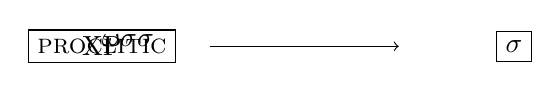
\begin{tikzpicture}[baseline]

    \Tree [ \node[draw]{{\textsc{proclitic}}}; [.\node(left){XP}; X ]]

    \begin{scope}[shift={(5cm,0cm)}]

    \Tree [.$\omega$ \node[draw](1){$\sigma$}; $\sigma$ $\sigma$ ]

    \end{scope}

    \draw [->, shorten >=1cm, shorten <=1cm] (left) to (1);

    \end{tikzpicture}
	 \hfill \citep[ex. 7]{Talic:2015}

\label{tal1}

\end{exe}

However, the clitic cannot interact with accent when syntactically attached  to
a  branching host. In this case, the latter forms a prosodic phrase (φ) to
which the proclitic may only attach.

\begin{exe}

	\ex
	\hfill
    \begin{tikzpicture}[baseline]
    \Tree [ \node[draw](1){\textsc{proclitic}}; [ NP {$\qquad$} ]]

    \begin{scope}[shift={(5cm, 0cm)}]

    \Tree [.φ \node[draw](2){$\sigma$}; [.$\omega$ $\sigma$ ]  ]

    \end{scope}

    \draw [->, shorten >=1cm, shorten <=2.25cm] (1) to (2);

    \end{tikzpicture}
	 \hfill \citep[ex. 8]{Talic:2015}

\label{tal2}
\end{exe}

Therefore, for the correct prosody to obtain, the syntactic configuration in
(\ref{tal1}) is required. Since under no approach can I derive such
base-generated constituency (recall the drawbacks), \citet{Talic:2015} assumes
that such orders are syntactically derived. In (\ref{tal3}), I show her
approach as demonstrated by her example (15) (ignoring the possibility of
secondary AP and converting the phrase marker into
\glsunset{BPS}\gls{BPS}).\is{bare phrase structure}

\begin{exe}
	\ex\label{tal3}
    
\begin{tikzpicture}[baseline=(root.base)]
        \Tree   [.\node(root){P\tsp{min}};
                    \node[draw]{P\tsp{min}};
                    [.\node(left){N\tsp{max}};
                        A\tsp{max}
                        N\tsp{max}
                    ]
                ]

        \begin{scope}[shift={(6cm, 0cm)}]

        \Tree   [.\node(root){P\tsp{max}};
                    [.\node(right){A$^{\text{max}}_{1}$};
                        P$^{\text{min}}_{2}$
                        A\tsp{min}
                    ]
                    [.P\tsp{min}
                        \emph{t}\tss{2}
                        [.N\tsp{max}
                            \emph{t}\tss{1}
                            N\tsp{max}
                        ]
                    ]
                ]

        \end{scope}

        \draw [->, shorten >=1cm, shorten <=1cm] (left) to (right);

        \end{tikzpicture}
\end{exe}

Such a syntactic approach assumes adjunct raising to Spec(root), viz.\
〈A$^\text{{max}}_{1}$, \emph{t}\tss{1}〉, and subsequent incorporation of
the preposition. This approach is architecturally rather similar to the
approach I developed, with one crucial exception. The chain
〈P$^{\text{min}}_{2}$, \emph{t}\tss{2}〉 can be seen as breaching the
anti-locality condition by moving the head into its own
specifier.\footnote{See~\cref{anti-loc}.} The author, however, adopts the lines
of reasoning from \citet{Matushansky:2006}, i.a., which are, on independent
grounds, divorced from the system of \citet{Roberts2010,roberts:2012uq} I am
building on.

Also note that the relation between the prosodic constituency property and the
availability of XLBE is not one of entailment. While the preposition \emph{u} I
have been citing in our data does have proclitic properties and is monosyllabic
(its syllabic $\omega$-weight: $\omega_\sigma(\textup{P}^{\text{min}})=1$)
there are other, prosodically non-simplex prepositions that feature in XLBE:\pagebreak

\begin{exe}
    \ex $\omega_\sigma(\textup{P}^{min})=2$
    (Ser-Bo-Croatian\il{Serbo-Croatian})\\
	\gll Prema velikoj je zgradi otišao.\\
	toward big.\Loc{} is building.\Loc{} went\\
	\trans `He went towards a big building.'

	\ex $\omega_\sigma(\textup{P}^{min})=3$
    (Ser-Bo-Croatian\il{Serbo-Croatian})\\
	\gll Povodom / uprkos teških je uslova ipak uspio. \\
        {in line} {} despite difficult.\Gen{} is circumstances.\Gen{} still succeeded \\
	\trans `Due to difficult circumstances, he still succeeded.'
\end{exe}

Thus, independently of the prosodic mappings, the anti-local configurations in
(\ref{tal3}) look as if, ceteris paribus, they should represent a standard
derivation of Ser-Bo-Croatian\il{Serbo-Croatian} PP grammar. Instead, I
proposed a non-violating derivation that maintains the approach in full format,
with little stipulation, and no reference to extra-syntactic
modules.\footnote{The end result is similar to one \citet{Boskovic:2005}
    achieves, being the only other account which achieves the required
constituency here, but the road to it is very different.}

\section{Phase-parameters of defective goalhood}
\label{sec:phase}

Following \citet{Chomsky2008} in assuming that only phase\is{phases} heads
trigger movement,  \citet{Roberts2010} concludes that phase\is{phases} heads
must, thereby, constitute the only cliticisation\is{clitics} sites. For the
clause, such phase\is{phases} heads are only C and \emph{v} and may adduce from
this idea of landing sites, or incorporation loci, a dichotomous typology of
pronominal cliticisation\is{clitics}: D-level arguments obligatorily cliticise
onto C$^0$, while φ-level pronouns target \emph{v}\tsp{0}, as outlined in
previous sections.

It is a fundamental requirement of the defectivity system that
\citet{Roberts2010} develops that lexical categorial features not constitute
formal features on which the notion of defectivity is defined.

Assume a configuration in which \emph{v}\tsp{0} combines with a φ-bearing
nominal element, $n^0$. According to the theory, the minimal noun, bearing
$[i\phi]$, incorporates\footnote{Or, rather, the feature valuation gives the
    effect of incorporation given that the chain reduction algorithm pronounces
    the copy at the head (effectively ``in'' \emph{v}\tsp{0}, by virtue of its
feature makeup).} into \emph{v}\tsp{0} after valuation of [\emph{u}φ] on the
latter. This is demonstrated in (\ref{inc1}). Assume, on the other hand, that
lexical categorial features constitute legitimately formal features: since
$[\textsc{n}]\neq[\textsc{v}]$, the condition on defectivity is not met in
(\ref{inc2}) and incorporation does not obtain. This is the problem I propose
to resolve.

\begin{multicols}{2}
	\tikzset{level distance=45pt,every tree node/.style={align=center,anchor=north}}
    \begin{exe}
    \ex F\tss{\emph{v}\tsp{0}} $\subset$ F\tss{\emph{n}\tsp{0}}\\
        \begin{tikzpicture}[baseline]
            \Tree
                [
                    [.{\emph{v}\tsp{0}\\{}[\sout{\emph{u}}φ]}
                        \node(1){\emph{n}\tsp{0}\\{}[\emph{i}φ]};
                        {\emph{v}\tsp{0}\\{}[\emph{\sout{u}}φ]}
                    ]
                    \edge [dashed]; [
                        [.\node(2){\tuple{$\begin{array}{c}n^0\\{}[\emph{i}$φ$]\end{array}$}};
                        ]
                        \edge [dashed]; {}
                    ]
                ]
             \draw[semithick, <-] (1.south)..controls +(south:1) and
             +(south:1).. node [fill=white] {\ding{51}} (2.south);

        \end{tikzpicture}%
        \label{inc1}
%    \columnbreak
     \ex F\tss{\emph{v}\tsp{0}} $\nsubset$ F\tss{\emph{n}\tsp{0}}\\
     \begin{tikzpicture}[baseline]
        \Tree
            [
                [.{\emph{v}\tsp{0}\\{}[\sout{\emph{u}}φ]}
                    \node(1){\emph{n}\tsp{0}\\[2mm]
                                $\begin{bmatrix}
                                    \textsc{n}\\
                                    \text{\emph{i}φ}
                                \end{bmatrix}$
                    };
                    {\emph{v}\tsp{0}\\[2mm]
                                $\begin{bmatrix}
                                    \textsc{v}\\
                                    \text{\sout{\emph{u}}φ}
                                \end{bmatrix}$
                    }
                ]
                \edge [dashed]; [
                    [.\node(2){\tuple{$\begin{array}{c}n^0\\
                                \begin{bmatrix}
                                    \textsc{n} \\
                                    \text{\emph{i}φ}
                                \end{bmatrix}\end{array}$}};
                    ]
                    \edge [dashed]; {}
                ]
            ]

        \draw[semithick, <-] (1.south)..controls +(south:1) and +(south:1)..
        node [fill=white] {\ding{55}} (2.south);

    \end{tikzpicture}%
    \label{inc2}
\end{exe}
\end{multicols}

For the principle of defectivity to be operational in its full generality, it
is necessary to develop the conditions under which both nominal and verbal
categorial (formal) features are subsets of a larger feature-class which would
legitimise (\ref{inc2}).

In this regard, I adopt the tenets that the lexical categorial features are
located in the categorisation formatives which combine with categoriless roots.
These are the standard assumptions of \isi{Distributed Morphology}.

Furthermore, it has been independently motivated that categorisers constitute
the First phase\is{phases}. I propose to treat categorisers as phasers more
explicitly. In this regard, I treat categorisers as \enquote{first-phasers},
with the nominal or verbal lexical category as their attribute.

\begin{exe}
\ex
\begin{xlista}
    \ex  $v^0 =_{\Def{}} \begin{bmatrix}π:\textsc{v}\end{bmatrix}$
    \ex  $n^0 =_{\Def{}} \begin{bmatrix}π:\textsc{n}\end{bmatrix}$
\end{xlista}
\end{exe}

What satisfies the defectivity condition in (\ref{inc2}) is that both the probe
and the goal bear the feature $[\pi]$, regardless of its (nominal or verbal)
attribute.

This alone derives the non-arbitrariness of the defectivity system, as
developed in \citet{Roberts2010}, which recognises and addresses only two
types of defective goals insofar as pronominal cliticisation\is{clitics} is concerned.\largerpage

\begin{exe}
	\ex
	\begin{xlista}
	\ex C-orientation:
	\begin{xlisti}
	\ex The relevant category of the \isi{defective goal} α: D/N
	\ex The category of the relevant probe β: C
    \ex\sloppy \isi{Agree} between phase-phase objects yielding incorporation via chain
        〈α\tss{[+π]}, α\tss{[+π]}〉
	\end{xlisti}
	\ex \emph{v}-orientation:
	\begin{xlisti}
	\ex The relevant category of the \isi{defective goal} α: φ
	\ex The category of the relevant probe β: \emph{v}
    \ex \isi{Agree} between phase-non-phase objects yielding incorporation via
    chain 〈α\tss{[+π]}, α\tss{[\textminus π]}〉
    \end{xlisti}	\end{xlista}
\end{exe}

My account leaves the analysis of \ili{Romance} pronominal
cliticisation\is{clitics}, which \textcite{Roberts2010} treats as involving a
defective φ goal and overall \emph{v}-orientation, untouched. What we are
allowing for is that the minimal D-less noun may count as a minimal
phase\is{phases} and, thus, as a \isi{defective goal} by virtue of
categorisation constituting a first phase\is{phases}.

Let me wrap up this section on a diachronic note and the question of the
historical sources of the D category in Slavonic as compared to, say,
\ili{Romance}.

\begin{exe}
	\ex
	\begin{xlista}
	\ex \ili{Romance} pronominal \isi{clitics} are φ-categories.
	\ex South Slavonic pronominal \isi{clitics} are N-categories.
	\end{xlista}
\end{exe}

Some varieties of South Slavonic (including \ili{Macedonian}, \ili{Bulgarian},
and, to some extent, \ili{Slovenian}) have developed an overtly full-fledged
D-category\linebreak which historically derives from demonstratives, in
contrast to Romance, where it derives from pronouns. Given the approach I just
outlined, the N/D parameter is therefore independent from the C-orientation
parameter for cliticisation.

%\subsection{The minimal phasehod of [D], [N], and [φ]}
%
%
%\begin{exe}
%\ex
%\begin{xlista}
%	\ex Pronominal cliticisation\is{clitics} in Ser-Bo-CroatiaMn is C-oriented.
%	\ex The \isi{defective goal} of the pronominal category is N.
%	\ex N-based pronouns are equally defective as D-based pronouns cross-linguistically \citep{Roberts2010}, given the N/D parameter.
%\end{xlista}
%\end{exe}
%
%Maybe a hierarchy of some kind?
%
%\begin{exe}
%\ex \Tree [.{Does the language project D?}
%[.no \edge[dashed]; {pronominal cliticisation\is{clitics} is C-oriented} ]
%[.yes \edge[dashed]; {D-cliticisation is \emph{v}-oriented} ] ]
%\end{exe}

\section{Discussion \& conclusion}

Let me take stock of the specific results this paper provides. The particular
goal was to derive a NS constituency-com\-pli\-ant analysis of XLBE and
\textsc{x2p}. To achieve this, I assumed an unrolling excorporation mechanism,
according to which all functional layers of the clause (and, inversely and
similarly, any other functional structure) originate as a complex head and
proceed to unroll and excorporate as each argument is introduced in the
structure. XLBE/\textsc{x2p} effects derive, as I have shown, from the featural
subset relation, which either holds or does not hold at the point when the
functional structure excorporates form the nominal category. In the last
section, I showed how the defectivity-driven approach to
cliticisation\is{clitics} is consistent with the N/D parametric theory which
assumes that some languages lack the functional D-layer. Assuming
categorisation is an attributive property of the first phase\is{phases}, I have
posited, on conceptually natural grounds, that phasality be recast as a feature
with categorial attributes. With this twist, the subset relation between N and
C categories can be established, and the N-clitics consistently treated as
C-orienting in South Slavonic.

The analysis I provided derives from basic properties of phrase-structure
building, coupled with the notion of defective goals and a derivational onset
as involving a head-complex \citep{Shimada:2007}. As it turns out, XLBE is
perfectly amenable to an exclusively syntactic account of its configuration,
thanks to \posscitet{Roberts2010} defectivity. A side product of such an
approach was also a desirable account of \textsc{2p} phenomena found in Bosnian
CSs, which feature the seeming \isi{movement} of the plural
auxiliary\is{auxiliaries} into the first conjuncts.

Such an approach may be a stepping stone to understanding the interaction of
pragmatics with speech act and vocative driven (X)LBE phenomena, as the
following one, which I leave for future research.

\begin{exe}
	\ex \gll $\Big[_{\emph{wish}\textup{P}}$ Sretan$_i$ ti, Ian-e, $t_i$ rođendan! $\Big]$ \\
    {}	happy.\M.\Sg{} you.\Dat{} Ian-\Voc{} {} birthday.\M.\Sg{} \\
    \trans	`Happy Birthday, Ian!'
\end{exe}

\printchapterglossary{}

{\sloppy\printbibliography[heading=subbibliography,notkeyword=this]}

\end{document}
